\documentclass {article}

\usepackage{graphicx}
\usepackage{amssymb}
\usepackage{amsmath}
\newcommand\conf{\mathbf{q}}
\newcommand\confoffset{\mathbf{q}_{off}}
\newcommand\transf[2]{^{#1}M_{#2}}
\newcommand\se[1]{\mathfrak{se}(#1)}
\newcommand\transl{\mathbf{t}}
\newcommand\linvel{\mathbf{v}}
\newcommand\angvel{\omega}
\newcommand\cross[1]{\left[#1\right]_{\times}}
\newcommand\x{\mathbf{x}}
\newcommand\y{\mathbf{y}}
\newcommand\hole{\mathbf{h}}
\newcommand\tool{\mathbf{t}}
\newcommand{\reals}{\mathbb{R}}

\title {Calibration of Pyrene arms and camera}
\author {Florent Lamiraux}
\date {}
\begin{document}
\maketitle
\section{Introduction}

\begin{figure}
  \centerline{
    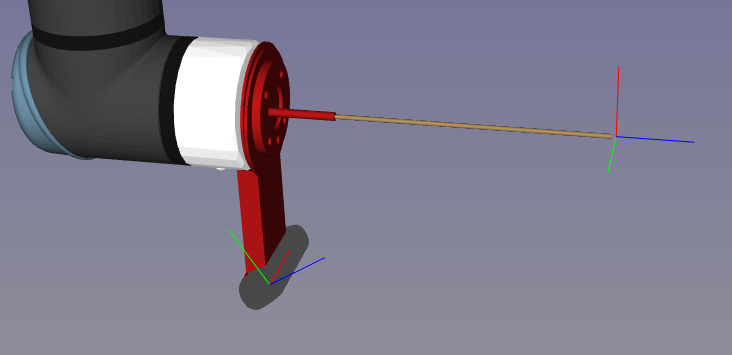
\includegraphics[width=.7\linewidth]{end-effector.png}
  }
  \caption{End effector with the tooltip and camera frames.}
  \label{fig:end-effector}
\end{figure}

The objective of this note is to process data collected with the UR10e robot
equipped with a camera in order to calibrate the pose of the camera and the position of the tooltip in the end effector frame.

\section{Calibration procedure}

The calibration procedure consists in two successive steps:
\begin{enumerate}
\item Calibrating the pose of the camera in the end effector frame,
\item calibrating the pose of the tooltip in the end effector frame.
\end{enumerate}

\subsection{Notation}

We denote by
\begin{itemize}
\item $\conf_1,\cdots,\conf_N$, $N$ calibration configurations,
\item $\transf{e}{c}\in SE(3)$ the pose of the camera in the end-effector frame. This
  is the unknown of the first step,
\item $\hat{\transf{c}{o}}^i\in SE(3)$ the pose of the part in the camera frame measured by the part localization software when the robot is in configuration $\conf_i$,
\item $^{o}\hole\in\reals^3$, the position of the hole in the part frame,
\item $\hat{\transf{c}{h}}^i = \hat{\transf{c}{o}}^i\, ^{o}\hole\in\reals^3$ the position of the hole in the camera frame, as measured by the localisation software,
\item $^{e}\tool$, the position of the tooltip in the end-effector frame,
\item $^{e}\hat{\Delta}_i$ the offset applied to align the tooltip with the hole in configuration $\conf_i$, expressed in the end-effector frame.
\end{itemize}

\subsection{Pose of the camera in the end effector frame}

The first step consists in generating a motion where the tool rotates in front
of a hole, stopping at 4 different orientations.

For each orientation, we use the \textit{tooltip calibration widget} to align
the tooltip with the hole and we save the data in a file.

For each measurement, we get the following equation:
$$
\transf{c}{e}(^e\tool + ^{e}\hat{\Delta}_i) - \hat{\transf{c}{h}}^i = 0
$$
The Jacobian of this equation with respect to $\transf{c}{e}$ is:
%% \begin{eqnarray*}
%%   \frac{d}{dt}(\transf{c}{e}(^e\tool + ^{e}\hat{\Delta}_i)) &=&
%%   \left(\begin{array}{cc}R\cross{\angvel} & R\linvel\\
%%     0 & 0\end{array}\right)
%%     \left(\begin{array}{c} ^e\tool + ^{e}\hat{\Delta}_i\\ 1\end{array}\right)\\
%%       &=& R\cross{\angvel}(^e\tool + ^{e}\hat{\Delta}_i) + R\linvel\\
%%       \left(\begin{array}{c}R \\ -R\cross{^e\tool + ^{e}\hat{\Delta}_i}\end{array}\right)&&
%% \end{eqnarray*}
$$
J = \left(\begin{array}{c} ^{c}R_{e} \\ -^{c}R_{e}\cross{^e\tool +\ ^{e}\hat{\Delta}_i}\end{array}\right)
$$
\subsection{Position of the tooltip in the end effector frame}


\end {document}
